\section{Definition of Coordination Operators between the TFSM and Activity Languages}

\begin{itemize}
	\item This section presents the \bcool specification of three operators between the TFSM and Activity languages: {SyncFSMEventsAndSignals}, \emph{startActivityWhenEnter} and {AtomicActivity}. In the following, we describe each operator and we discuss their semantics. We then present the \bcool specification according with the chosen semantics.  
	
	\item The \emph{SyncFSMEventsAndSignals} operator differs from the running example operator because it synchronizes FSMEvents and Signals. Whereas in the running example the occurrences of FSMEvents were synchronized with the starting of Actions, here they are synchronized with the occurrences of Signals, \ie by coordinating instances of \dse \emph{occurs} and \emph{signalOccurs}. This operator only requires a slight modification of the specification presented in the running example (see Listing~\ref{lst:bcoolrunningexample}). The only modification is the type of the \dse used in the operator (see Listing~\ref{lst:bcoolsigandfsmevents}: line 1). The rest of the definition (\ie the correspondence matching and coordination rule) is unchanged (see Listing~\ref{lst:bcoolsigandfsmevents}: line 2 and 3). We want to highlight that the adaptation has been done only by identifying the new \dse to be constrained. This should also be the case for other coordination pattern.
	

	 
\begin{lstlisting}[language=bcool,
caption={\bcool specification of the \emph{SyncFSMEventsAndSignals} operator},
label={lst:bcoolsigandfsmevents}, 
basicstyle=\scriptsize\ttfamily, backgroundcolor=\color{LGrey}, numbers=left, xleftmargin=2pt]
Operator SyncFSMEventsAndSignals(SignalOccurs:activity::signalOccurs, FSMEventOccurs:tfsm::occurs)
when (SignalOccurs.name = FSMEventOccurs.name);
do   RendezVous(SignalOccurs, FSMEventOccurs)
end operator
\end{lstlisting}
	 
	 
	 
	 \item The \emph{startActivityWhenEnter} operator specifies a hierarchical coordination pattern between the TFSM and Activity languages, unlike hierarchical coordination frameworks where the semantics is hidden, this operator explicitly specifies how the hierarchical coordination is implemented. In our case, we chose the semantics in which entering in a specific state of a TFSM model triggers the execution of a given Activity. When leaving a state, several semantic variation points may be chosen. The outgoing transitions from a state can be considered, for instance, as preemptive for the activity model (\ie firing a transition from a state to another preempts the internal activity). Alternatively, the transition can be considered as non-preemptive (\ie the states cannot be left before the associated activity finishes). In our case, we chose non-preemptive transitions because the activity should not be interrupted until the information has been sent. Thus, we ensure that the activity executes at least one time.  
	
	
	 \item We define the \emph{startActivityWhenEnter} (Listing~\ref{lst:bcoolStartActivityWhenEnter}: line 1) operator that coordinates the entering and leaving of a state with the execution of an activity. The entering into a state is identified by the \dse \textit{entering} defined in the context of State. Instances of such \dse have to be coordinated with instances of the \dse \textit{startActivity}. Similarly, leaving a state is identified by \dse \textit{leaving} and finishing an activity is identified by \dse \textit{finishActivity}. To identify pairs of such events, the correspondence matching selects instances of \dse \emph{startActivity} and \emph{finishActivity} by using their context (Listing~\ref{lst:bcoolStartActivityWhenEnter}: line 2). The pairs selected identify the starting and finishing of the same activity. Besides, we select the activities that represent a state by comparing the \emph{onEnterAction} defined in the states and the name of the activities. OnEnterAction is a string defined in the context of State (see Figure~\ref{fig:tfsmmm}) that specifies the method invoked when a state is entered. In our case, we use this attribute to specify the name of the activity that the state represents (Listing~\ref{lst:bcoolStartActivityWhenEnter}: line 2).
	
	 
	 \begin{lstlisting}[language=bcool,
	 caption={Hierarchical operator between TFSM and Activity languages},
	 label={lst:bcoolStartActivityWhenEnter}, 
	 basicstyle=\scriptsize\ttfamily, backgroundcolor=\color{LGrey}, numbers=left, xleftmargin=2pt]
	 Operator  startActivityWhenEnter (activityStart : ad::startActivity , activityStop : ad::finishActivity, enterState : tfsm::entering, leaveState : tfsm::leaving)
	 when ((activityStart = activityStop) and (enterState = leaveState) and (activityStart.name = enterState.onEnterAction));
	 do 
		 ExecuteActivityNonPeemptive (enterState, leaveState, activityStart, activityStop)
	 end operator;
	 \end{lstlisting}
	 
	 \item To coordinate the selected instances of \dse, the coordination rule uses the event relation \emph{ExecuteActivityNonPeemptive}, which is defined in \moccml (see Figure~\ref{fig:looprelation}). The relation takes four events as parameters: the events \emph{modeEnter} and \emph{modeLeave} that represents respectively the entering and leaving of a state; and the events \emph{startActivity} and \emph{finishActivity} that represents respectively the starting and finishing of an activity. The state-based representation is made of two states named \emph{waitEnterState} and \emph{WaitFinishActivity}. In waitEnterState state, the events modeEnter, modeLeave and startActivity are allowed to tick. Only when modeEnter and startActivity happen simultaneously, the state \emph{waitFinishActivity} is reached. In this state, only the finishActivity is allowed to happen. When this event occurs, \ie the activity has finished, the state \emph{waitEnterState} is reached and the modeLeave is allowed to occur. The use of this relation in the coordination rule results in transitions that cannot preempt the execution of the internal activities. The entering a state makes the activity to start to execute synchronously. Then, only after the activity has finished, the state can be left.
	 
	 \item We want to highlight that an integrator can vary the semantics of the coordination by only modifying the event relation in the coordination rule. For instance, by modifying the event relation, the transition may become preemptive.
	 
	 \todo{todomoccmlpicture}
	 \begin{figure}[h]
	 	\center
	 	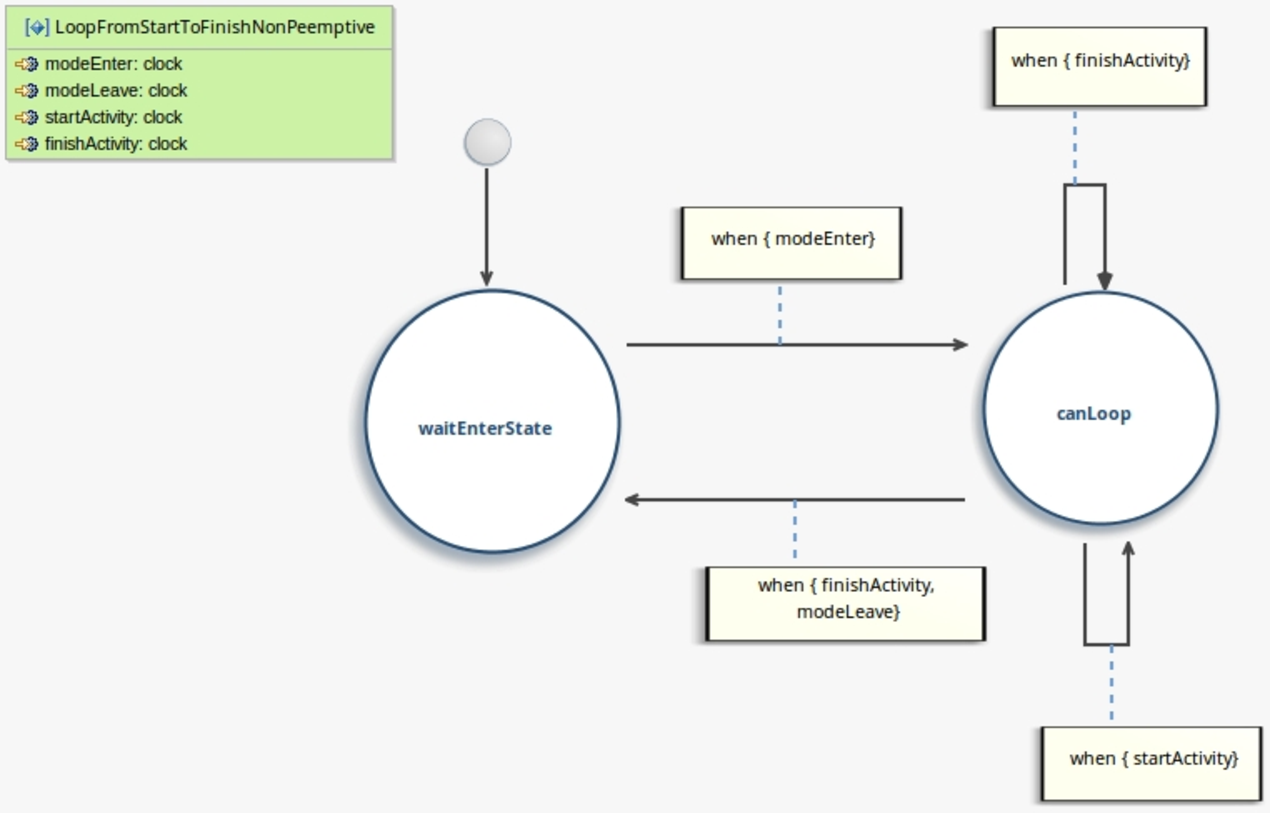
\includegraphics[width=.7\columnwidth]{examples/figs/LoopFromStartToFinishNonPreemptive}
	 	\caption{\emph{ExecuteActivityNonPeemptive} event relation}
	 	\label{fig:looprelation}
	 \end{figure}
	 
	
	 \item In the \emph{AtomicActivity} operator, we deal with the temporal aspects of the model coordination. The operator specifies how the time in the TFSM elapses during the execution of an activity. In these languages, the time is represented differently. In the TFSM language, each state machine has a \emph{localClock} used to measure the time while the Activity language is untimed. The local clock is a \emph{FSMClock}, which defines a \dse named \emph{ticks} whose occurrences represent a physical time increment. In the Activity language, the duration of activities can be represented as the time between the \dse \emph{startActivity} and \dse \emph{finishActivity}. To coordinate the time, it is necessary to specify the number of \emph{ticks} of the local clock between the occurrence of the \dse \emph{startActivity} and \emph{finishActivity}. Again, several semantic variation points may be chose. For instance, the coordination rule could express that the execution of the activities takes a fixed amount of time. In our example, we propose to enforce the execution of the activity to be atomic with respect to the time in the TFSM model. As a result, there are no occurrences of the \dse ticks of the corresponding local clock during the execution of the activity.
	 
	 
	 \item In \bcool, we define the operator \emph{AtomicActivity} (Listing~\ref{lst:bcoolAtomicExec}: line 6) that specifies how time is consumed during the execution of the activities. The correspondence matching selects instances of \dse \emph{startActivity} and \emph{finishActivity} by using their context. Thus, it selects the instances that belong to the same activity. Note that the correspondence matching does not filter instances of \dse \emph{ticks}, as a result, the selected activities will be atomic respect to all the clocks in the TFSM. However, the TFSM language forces to one the number of localClocks in a TFSM. Thus, there is only one instance of \dse \emph{ticks} in each TFSM. 
	 
	 
	 \begin{lstlisting}[language=bcool,
	 caption={Timing operator between TFSM and Activity languages},
	 label={lst:bcoolAtomicExec}, 
	 basicstyle=\scriptsize\ttfamily, backgroundcolor=\color{LGrey}, numbers=left, xleftmargin=2pt, firstnumber=6]
	 Operator AtomicActivity (activityStart : ad::startActivity , activityStop : ad::finishActivity, timeTicks : tfsm::ticks)
	 when (activityStart = activityStop );
	 do 
		 AtomicExec (activityStart, activityStop, timeTicks)
	 end operator;
	 \end{lstlisting}
	 
	 
	 \item To express the coordination rule, we use the event relation \emph{AtomicExec} which makes the execution of the activities atomic with respect to the local clock of the TFSM (see Figure~\ref{fig:atomicexec}). The event relation accepts three events as parameters: \emph{ticks}, \emph{startAct} and \emph{finishAct}. While the event ticks represents the ticking of the local clock, the startAct and finishAct events represent respectively the starting and finishing of an activity. In \emph{waitstartActivity} state, the event ticks is allowed to occur, thus making the time elapse. When the startAct event happens, \ie the activity starts to execute, the \emph{waitfinishActivity} state is reached and the event ticks is forbidden to occur, \ie the time in the TFSM does not elapse while the activity executes. Only when the event finishAct happens, the \emph{waitstartActivity} state is reached, and \emph{ticks} is allowed to occur again. In the operator, we use this relation to make the execution of the activities atomic, \ie there is no occurrence of the \dse ticks of the corresponding local clock during the execution of the activity.
	 
	 \todo{todomoccmlpicture}
	 
	 \begin{figure}
	 	\center
	 	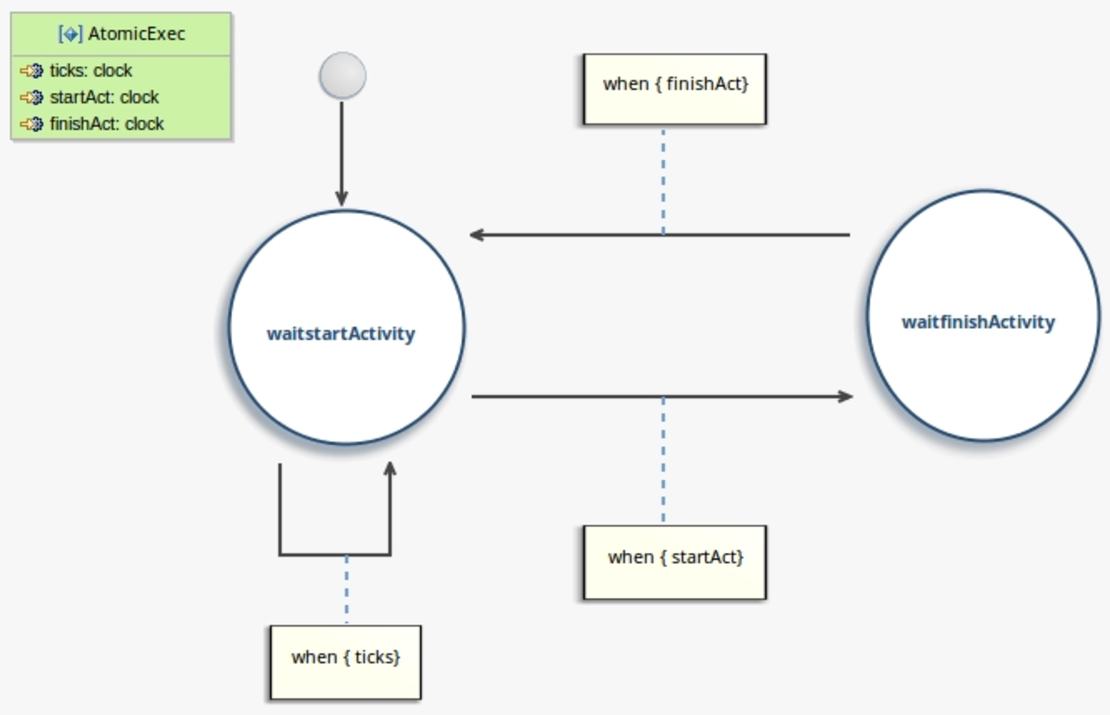
\includegraphics[width=.7\columnwidth]{examples/figs/AtomicExec}
	 	\caption{\emph{AtomicActivity} event relation}
	 	\label{fig:atomicexec}
	 \end{figure}
	 
	 
	 
	 \item In this section, we have used \bcool to define a set of coordination operators that deal with both control and timing aspects of the coordination between TFSM and Activity languages. Unlike hierarchical coordination frameworks where the semantics is hidden, these operators explicitly specified how the coordination is implemented. More precisely, coordination rules explicitly define the semantics of the resulting coordination. Furthermore, we ease the definition of relations by using \moccml, a dedicated language to express constraints between events. Thus, an integrator can vary the semantics of the coordination by only modifying the event relation in the coordination rule. Frameworks like Ptolemy do not support such a variation without changing the current implementation of the framework. This means modifying the implementation of a \emph{director} written in Java, which needs a good knowledge of the framework. In our approach, we are using a language dedicated to language integrator experts thus easing the understanding and adaptation of the \bcool specification. In the next section, we use these operators to coordinate and execute the models of the surveillance camera system.
	 
\end{itemize}


  










%Similar than the \emph{startActivityWhenEnter} operator, the \emph{AtomicActivity} operator also defines a coordination between states and activities, but in this case, it deals with the temporal aspects of the coordination. The operator specifies how the time in the TFSM elapses during the execution of the activities that specify the on-entry action of a state. Thus, this coordination is also hierarchical, but in this case, only considers the timing aspects. %In these languages, the time is represented differently. In the TFSM language, each state machine has a \emph{localClock} used to measure the time while the Activity language is untimed. The local clock is a \emph{FSMClock}, which defines a \dse named \emph{ticks} whose occurrences represent a physical time increment. In the Activity language, the duration of activities can be represented as the time between the \dse \emph{startActivity} and \dse \emph{finishActivity}. Thus, to coordinate the time, it is necessary to specify the number of \emph{ticks} of the local clock between the occurrence of the \dse \emph{startActivity} and \emph{finishActivity}. In this operator, we propose to enforce the execution of the ``internal'' activity to be atomic with respect to the time in the TFSM model. As a result, there is no occurrence of the \dse ticks of the corresponding local clock during the execution of the activity. 










